\documentclass[12pt]{article}
\usepackage[utf8]{inputenc}

\title{Challenging \cv to a Functional Language}
\author{CS 6140 (ML): Project Proposal}
\date{}%October 2019}

\usepackage{amsmath}
\usepackage{amsfonts}
\usepackage{fullpage}
\usepackage{enumitem}
\usepackage{url}
\usepackage{hyperref}
\usepackage{tikz}
%\usepackage{booktabs}

\usepackage{setspace}
\usepackage[margin=1in]{geometry}
\onehalfspacing

\usepackage{xcolor}
\usepackage{xspace}

\usepackage{nicefrac}

\usepackage[numbers]{natbib}

\newcommand{\head}[1]{%
\noindent\fbox{%
\parbox{\linewidth}{%
{\bf CS6140: Machine Learning}
\begin{center}
\Large Homework Assignment \# #1
\end{center}
{\it Yulia Belyakova}\hfill\url{belyakova.y@northeastern.edu}\\
{\it Artem Pelenitsyn}\hfill\url{pelenitsyn.a@northeastern.edu}
}}
\vspace{1mm}
}

\renewcommand{\thesubsection}{(\alph{subsection})}

\newcommand{\cv}{\texttt{code2vec}\xspace}
\newcommand{\csharp}{C\texttt{\#}\xspace}
\newcommand{\cpp}{C\texttt{++}\xspace}

\newcommand{\todo}[1]{\textbf{TODO[}#1\textbf{]}}
\newcommand{\defn}[1]{\textbf{#1}}

\newcommand{\uhref}[2]{\underline{\href{#1}{#2}}}


\begin{document}

\head 3

{\let\newpage\relax\maketitle}

\section{Objectives and Significance}

%(1-2 paragraphs)
%(a) Describe what the goal of the project is, why is it important, and your motivation for doing it.

% could use some motivation from survey of ML4PL 2018
% https://miltos.allamanis.com/publicationfiles/allamanis2018survey/allamanis2018survey.pdf

Descriptive and consistent names of routines serve at least two goals:
(1)~improve code readability and maintainability, 
and (2)~facilitate better public APIs%
\footnote{Application Programming Interface},
as the library users often search for a routine by a name.
But coming with a good name agreed upon by other programmers can be hard.
%Coming up with a good name might be hard, 
%but it is even harder to pick the name that other people consider good too.
Thus, programmers would benefit from an automatic tool 
that suggests names according to the best practices and naming conventions.

As there are loads of open source projects, there is an opportunity
to use machine learning for extracting and predicting descriptive 
method names~\cite{Allamanis2015,Alon2018,code2vec}.
To the best of our knowledge, so far research in this area has been focused 
on object-oriented languages, including Java, Python, and JavaScript.
We are interested in testing the idea in a different context~--- 
that of a functional language. 

The goal of our work is to challenge the \cv framework,
a neural model for predicting method names, published at POPL 2019~\cite{code2vec}.
We want to find out whether \cv can accurately predict
function names (instead of method names) in the context
of a language with higher-order functions,
algebraic datatypes, and pattern matching.
We pick the Haskell programming language as a representative example
of functional languages.



%========================================================
\section{Background}
%(1-2 pages)

\subsection{Concepts}

\defn{Routine} (function, method) is a \emph{named}, reusable code snippet designed to perform a specific task.
Different software projects can define similar or even identical routines.
Ideally, all routines that serve the same goal should have the same name.
Therefore, the best name for a routine would be the one used the most for the same problem.
In general, it is impossible to know whether two routines solve the same problem
(i.e. have the same semantics), 
but if the code is well-structured and short enough, 
a human can answer this question by simply inspecting the code;
a \textit{name-predicting tool} should be able to do the same on a large scale.

%\paragraph{(a) Introduce all important concepts and background information}

\defn{AST} (Abstract Syntax Tree) is a tree representation of program code where each node denotes
a construct from the program (see example in Fig.\,\ref{fig:ast}).
Given a programming language and a text of a program written in it, 
it is relatively straightforward
to transform the text into a tree (parse the program). 
Building AST is the first step in most compilers.

\begin{figure}
\centering
\begin{minipage}{5cm}
\begin{verbatim}
    while true
        x := x + 1
    end
\end{verbatim}
\end{minipage}
\begin{minipage}{6cm}
\centering
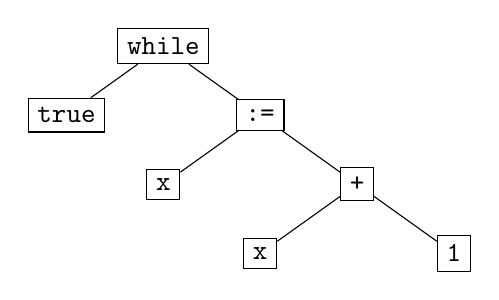
\begin{tikzpicture}[sibling distance=7em, level distance=2.5em,
    concrete/.style = {shape=rectangle, draw, align=center}]
\node[concrete] {\texttt{while}}
child { node[concrete] {\texttt{true}} }
child { node[concrete] {\texttt{:=}}
	child { node[concrete] {\texttt{x}} }
	child { 
	    node[concrete] {\texttt{+}}
	    child { node[concrete] {\texttt{x}} }
	    child { node[concrete] {\texttt{1}} } }
	}
;
\end{tikzpicture}
\end{minipage}
%\includegraphics[height=5cm]{ast.png}
    \caption{An Example of AST}
    \label{fig:ast}
\end{figure}
  
\defn{Higher-order function} is a function that accepts another function as an argument
or returns a function as a result. For example, the function \texttt{double(f, x) = f(f(x))}
is higher-order: its first argument \texttt{f} is itself a function, 
and \texttt{double} calls \texttt{f} twice.

\subsection{Related Work and Motivation}

%\paragraph{(b) Search the literature and describe previous work on this problem}
%The idea of using paths to do code embedding appeared in~\cite{Allamanis2015}.

%\paragraph{(c) If there exists previous work on the problem, describe what makes your work distinct or particularly interesting}

There have been multiple attempts to apply machine learning techniques
to computer programs. The major challenge here is to represent a code snippet
in a way that is both tractable by learning algorithms but also meaningful.
One approach is to treat code as text in a natural language
and apply natural languages processing (NLP) techniques~--- the, so called, 
naturalness hypothesis~\cite{Allamanis2018}. The advantage of the approach
is its simplicity, but on the downside, the information 
about the hierarchical nature of the code is totally lost.
Therefore, instead of representing a program as a sequence of tokens,
one can alternatively look at its abstract syntax tree (AST)~\cite{Raychev2016,Allamanis2018}.
Recently,~\citet{Alon2018} introduced the \emph{path-based} approach, 
which considers leaf-to-leaf paths on the program AST.
Based on that, \citet{code2vec} developed a method of aggregating the paths
into a single fixed-length \emph{code vector}, 
thus making a \defn{code embedding}~\cite{Allamanis2015}.

Code embeddings enable the application of various machine learning techniques 
in the field of programming languages.
In particular, the \cv framework~\cite{code2vec} implements a neural model
that uses code vectors to predict method names for the Java and \csharp programming languages,
with extensions of \cv\footnote{
\scriptsize\url{https://github.com/tech-srl/code2vec/blob/master/README.md\#extending-to-other-languages}} 
targeting Python and C/\cpp.
The authors' previous work~\cite{Alon2018} had support for predicting
variable names and types of expressions in Java, \csharp, Python, and JavaScript,
though this functionality is not supported by \cv.

While the variance of the names prediction accuracy across the \emph{supported} languages 
is about only~10\%, to the best of our knowledge, 
no one has attempted to implement code embeddings for \emph{functional} languages.
They support features not typical for languages such as Java or Python,
for instance, algebraic data types and pattern matching,
so we have to find a way to turn them into paths efficiently.
Furthermore, functional programs tend to use higher-order functions more
than object-oriented programs use higher-order methods.
Therefore, we suspect that this might affect the performance of the \cv approach.

%========================================================
\section{Proposed Approach}
%(2-4 pages)

\subsection{Data Acquisition}

To train a \cv model for the Haskell language, we need to obtain a large amount of code on that language.
For this, we will use
Hackage%
\footnote{\url{http://hackage.haskell.org/}},
a centralized curated set of Haskell packages.
The set consists of $\sim$16 thousand packages with source code available. Hackage has 
both web interface and a command-line tool to fetch its packages. We are going to implement
a Shell script that would query the whole list of packages and download every package from that list.

The enormous amount of code duplication in public code repositories~\cite{Lopes2017} is a clear threat 
to ML applications to big code. We conjecture that a curated set of packages, such as Hackage, should 
be less of a victim to the threat. This line of reasoning is applied in~\cite{code2vec} too: the authors
take top GitHub projects in the hope that ``popular'' projects are not (as much) susceptible to the 
duplication problem.

Preliminary experiments and anecdotal evidence suggest several gigabytes of source code on Hackage
if consider only the latest versions of the packages (to avoid duplication). 
While the latest \cv work~\cite{code2vec} 
operated on tens of gigabytes of Java files, \citet{Allamanis2018} used about 5 gigabytes of code when
working with other languages. Thus, we hope that the code from Hackage will allow us to build a useful model.

\subsection{Proposed Method and Implementation}

Our goal is to add the support for Haskell into the \cv framework.
%
The paper on \cv has been published along the artifact freely available on GitHub\footnote{
\url{https://github.com/tech-srl/code2vec/}}. In
the README file of the GitHub repository, the authors left several notes on extending 
their project to analysing different programming languages. In a nutshell, adding 
support for a new language amounts to writing an \emph{extractor} — a tool capable of 
extracting path information out of source code. Typically, an extractor will use a parser
for corresponding programming language to get an AST of a code snippet. 
Then, the AST is used by the extractor to generate paths and dump them into the simple textual 
format expected by \cv.

One challenge in building an extractor is to find a parser for the language of interest.
Fortunately, in the case of Haskell, we have one major compiler for the language, the GHC compiler, 
which supplies its parsing engine in the form of a package (located on Hackage).
% ?link to http://hackage.haskell.org/package/ghc-lib-parser

Another challenge for path-based code embedding is the amount of paths encoded in AST.
Even a simplest program written on any programming language can hold a multitude of paths. 
The authors of the \cv work 
identified a feasible cutoff point for discarding paths; this is done using
particular properties of the paths.
We need to come up with reasonable threshold values too, and 
make sure that those numbers allow for teaching a useful model given limited computational resources.

Provided the paths are successfully generated for the training set,
the \cv framework can be configured to use these data for training a model.
The next step is evaluation of the model.

\subsection{Evaluation Strategy}

Given a Haskell code snippet, the model yields a label — the proposed name for the snippet.
If the snippet originated from a real function, we know the true label for it, and, therefore, can 
determine true and false positives.
Given those outcomes, 
the accuracy of labelling can be measured using several well-known statistics, namely: \textit{precision}
(number of true positives divided by the total number of elements labeled), \textit{recall} (the number 
of true positives divided by the total number of elements that actually belong to the positive class) 
and a combination of them called \textit{F1 score}:
\[
    F_1 = 2 \cdot \frac 
        {\text{precision}\cdot\text{recall}}
        {\text{precision} + \text{recall}}.
\]
In fact, the original \cv work~\cite{code2vec} used all three to asses the quality of their model. 
We are going
to reuse the metrics for evaluating our project. This enables us to compare the performance of our model 
to the one built for Java in~\cite{code2vec}.

The experiment will require dividing the data set into training, 
validation and testing subsets, as is accustomed.
%
The validation subset is used in~\cite{code2vec} to tune 
hyperparameters concerning the cutoff value for the paths to be considered. 
%
Following~\cite{Allamanis2018}, we plan to randomly pick 80--90\% of the data set for training, and
divide the rest between validation and testing sets evenly, as in~\cite{code2vec}.


\subsection{Expected Outcomes and Fallback Option}

Our goal is to obtain a model for predicting function names for Haskell code snippets. The model should achieve 
reasonable performance by the measures described above. As already mentioned, our
project has several threats to validity:
\begin{itemize}
    \item smaller raw data set (compared to~\cite{code2vec}),
    \item less of computational resources,
    \item less time to experiment with cutoff values,
    \item unique features of functional languages not targeted by the initial work.
\end{itemize}

Given the challenges we face, we might not achieve the goal. We think that it would be an interesting 
outcome on its own, suggesting that functional languages require some substantial changes in
the \cv approach.
In that scenario, we are willing to 
explore a simpler application of code embedding, namely, finding similar code snippets. 
We conjecture that proximate code vectors could suggest code clones (or near-clones).
Using clustering, we hope to detect code duplicates in automated fashion.

\section{Individual tasks}
%(1-3 paragraphs)

%\textbf{Describe what each member of the team will do and justify why each person is necessary. In
%the project report (at the end of semester) you will have to be specific about what each person
%actually contributed to the project.}

We decided to divide the work as follows:

\begin{itemize}
    \item getting the data from Hackage — Artem;
    \item cleaning and preparing the data (filtering and shuffling Haskell source files) — Julia;
    \item extracting ASTs using GHC's parser — Artem;
    \item extracting paths from ASTs — Julia;
    \item piping extracted paths to \cv and training the model — Artem; % on server hardware
    \item validation: experimenting the resulting model, tuning hyperparameters — together;
    \item testing: measuring accuracy --- together;
    \item writing final report --- each person covers their corresponding job.
\end{itemize}

% (b) If the project is a part or extension of some other project you have carried out (or will), explain
% all relevant details and what is the work that differs from what you already have done or are doing
% for another purpose.
% ^ NA

\bibliographystyle{unsrtnat}
\bibliography{refs}

\end{document}
